
\begin{figure}[t!]
\begin{center}
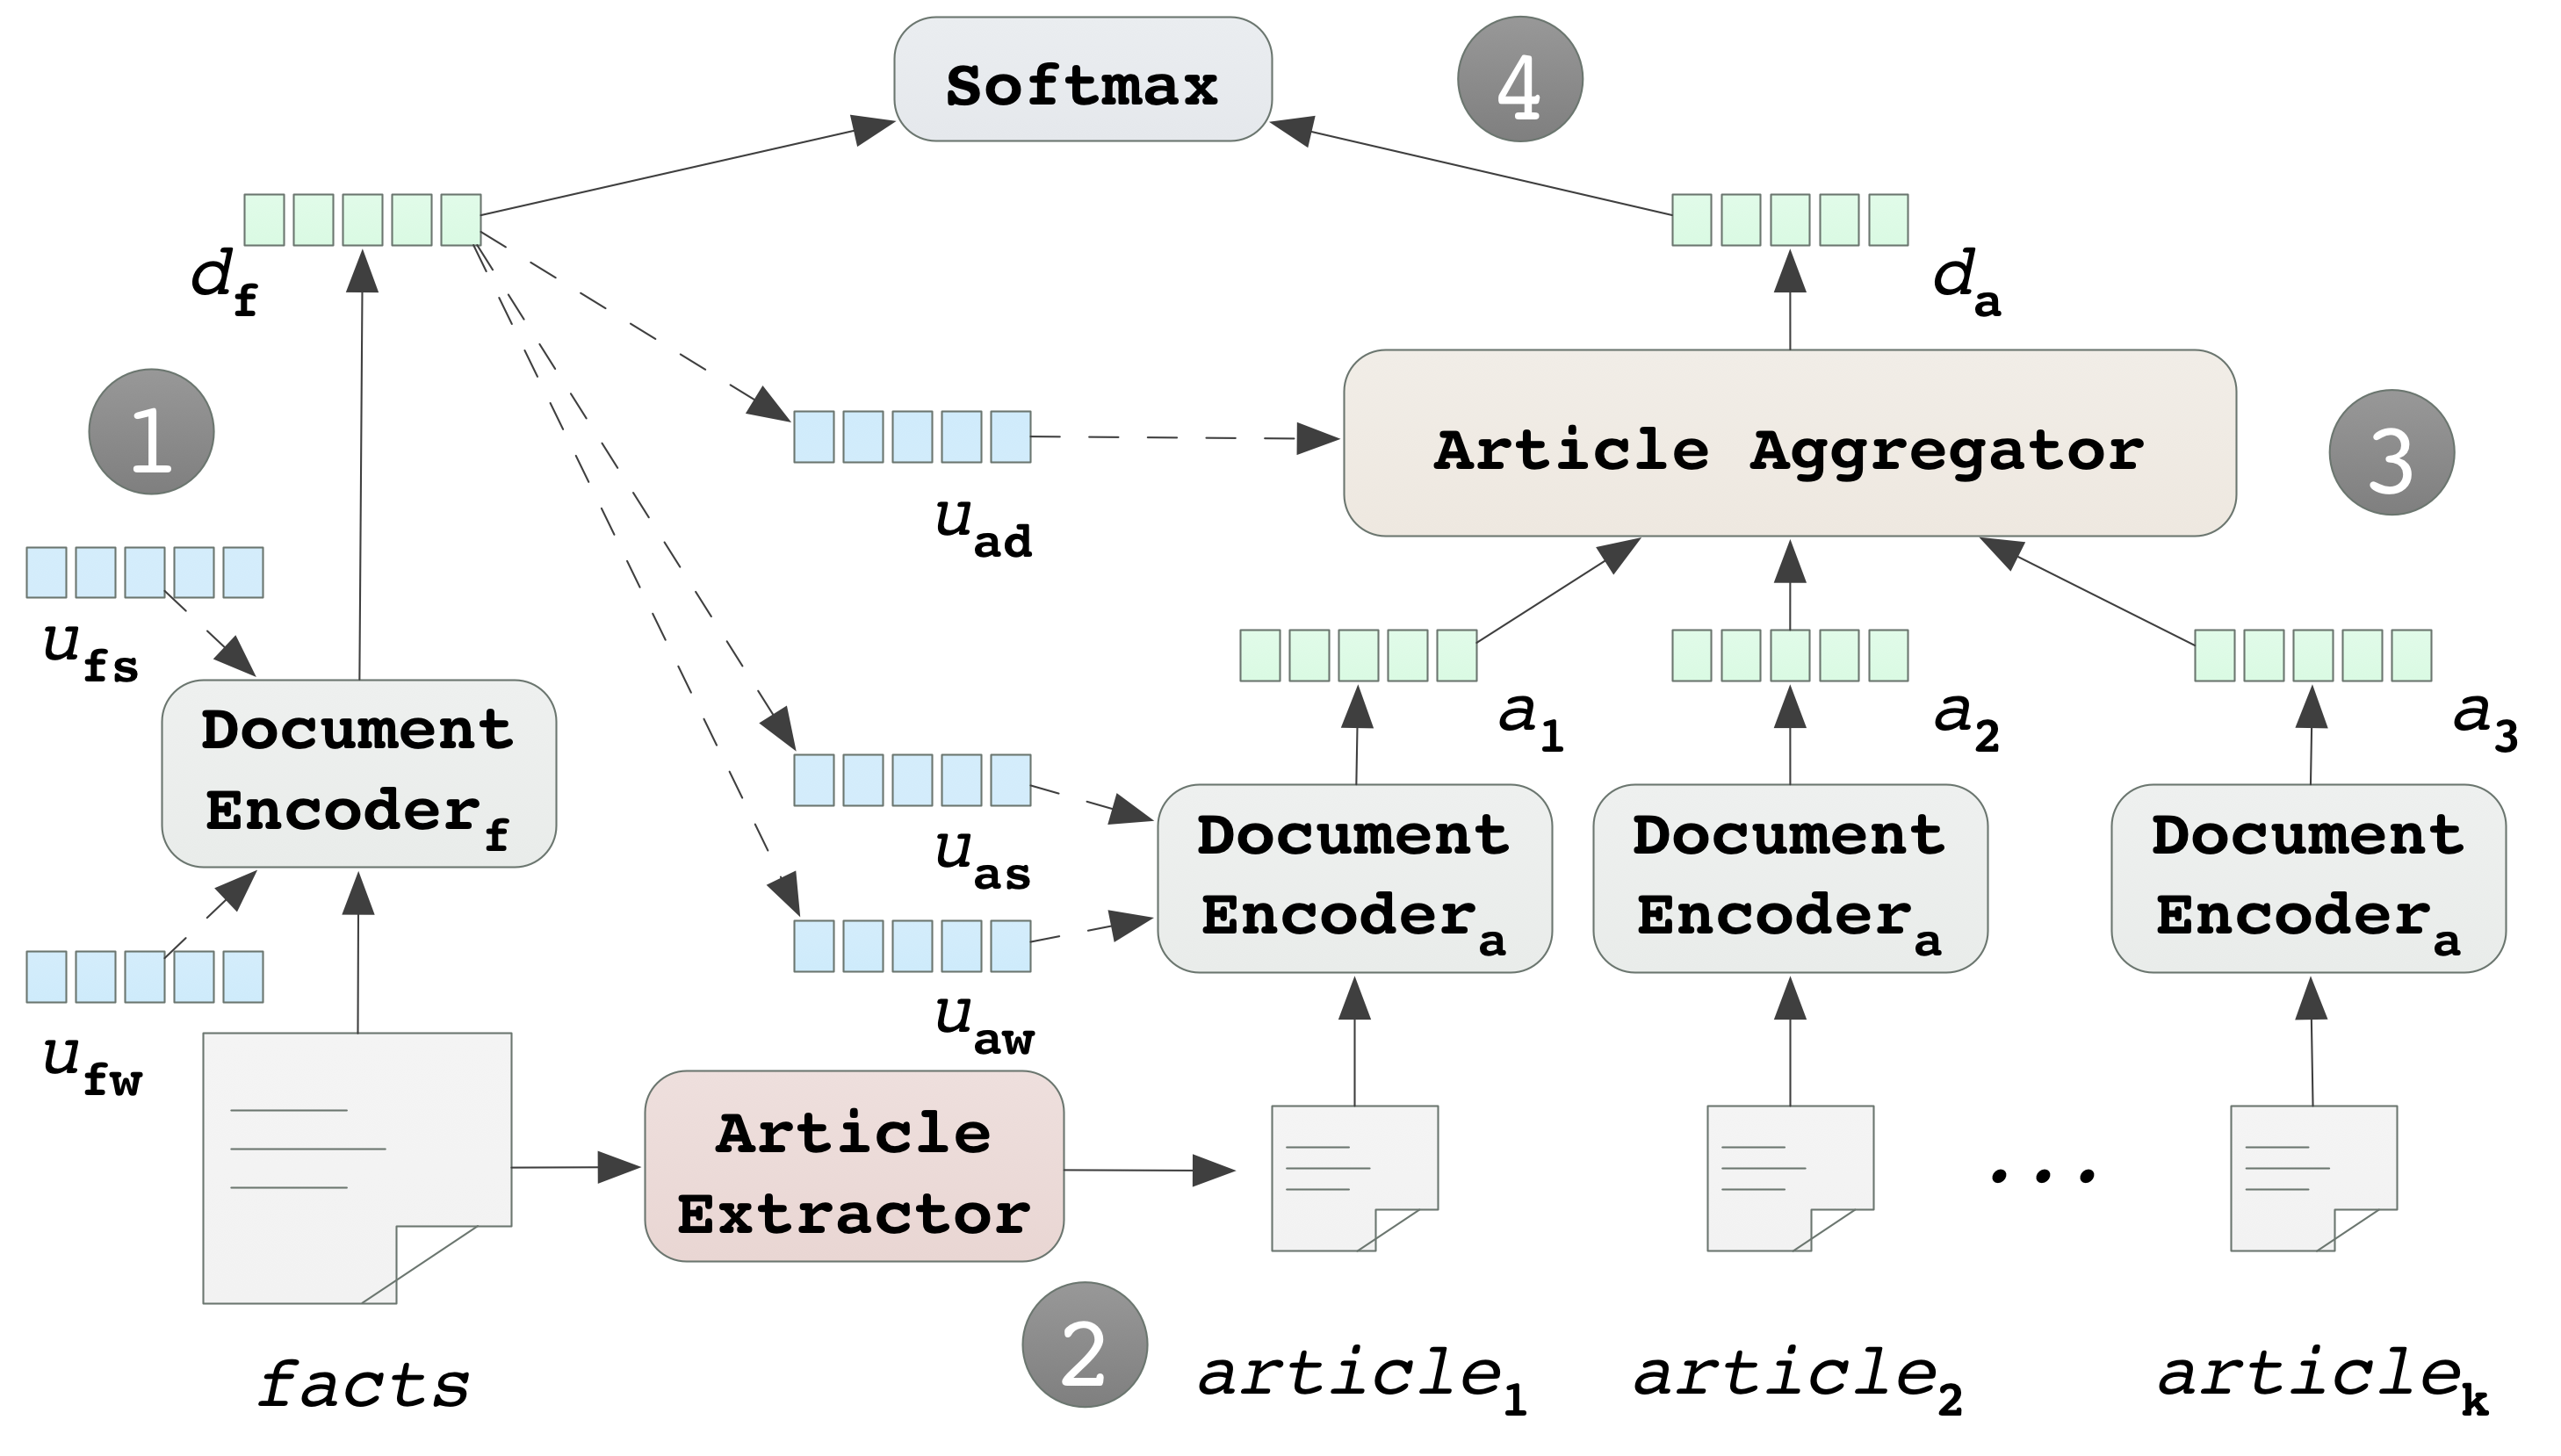
\includegraphics[width=0.48\textwidth]{figures/charge_pred_overview.png}	
\caption{Overview of Our Model}
\label{fig_model_framework}
\end{center}
\end{figure}

\section{Our Approach}
% In order to generate reasonable charge prediction, 
Our approach follows four steps as depicted in Figure \ref{fig_model_framework}. 
(1) The input fact description is fed to a document encoder to generate the fact embedding $\mathbf{d_f}$.
(2) Concurrently, the fact description is also passed to an article extractor to find top $k$ relevant law articles. 
(3) The extracted articles are fed to another document encoder, and the resultant article embeddings are passed to an article aggregator to produce the aggregated article embedding $\mathbf{d_a}$. Meanwhile, three context vectors, i.e., $\mathbf{u_{aw}}$, $\mathbf{u_{as}}$ and $\mathbf{u_{ad}}$, are dynamically generated from $\mathbf{d_f}$ for the article document encoder and the article aggregator. 
(4) Finally, $\mathbf{d_f}$ and $\mathbf{d_a}$ are concatenated and passed to a softmax classifier to predict the charge distribution for the input case.

%The fact-based charge classification task can be formatted as a multi-label document classification task. The input is several sentences describing the facts of a case, and the output is multiple charges related to the case. Since usually multiple elements are required to constitute a charge (for example, the charge of acceptance of bribes requires the defendant to illegally accepts another person's money, and the defendant should also be a state functionary), the recurrent neural network (RNN) seems like a natural fit for the task. Considering the fact that only a small portion of the facts are crucial for the determination of charges, we also use attention mechanism in our model. Since the HAN model  satisfies many of our requirements except the multi-label classification capability, we use the framework of the HAN model for document embedding, but replace the output module and the loss function with ones that are compatible with the multi-label classification task. Furthermore, to take the information of article into account, we add another article attention module to incorporate the information of relevant articles to the model.

\subsection{Document Encoder}
\label{sec_doc_encoder}
% Our document encoder module is based on the framework of Hierarchical Neural Network (HAN) proposed by \cite{yang2016hierarchical}. The overview of our document encoder is shown in Figure \ref{fig_doc_encoder}. 
Intuitively, a sentence is a sequence of words and a document is a sequence of sentences. As suggested by \cite{tang2015document,yang2016hierarchical}, the document embedding problem can be converted to two sequence embedding problems. As shown in Figure \ref{fig_doc_encoder}, we can first embed each sentence using a sentence-level sequence encoder, and then aggregate them with a document-level sequence encoder to generate the document embedding $\mathbf{d}$. 
% Therefore, the key problem of document embedding converts to building an effective sequence encoder.
Although it is possible to use different models for these two sequence encoders, we simply use the same architecture here for simplicity.

\begin{figure}[htbp]
\begin{center}
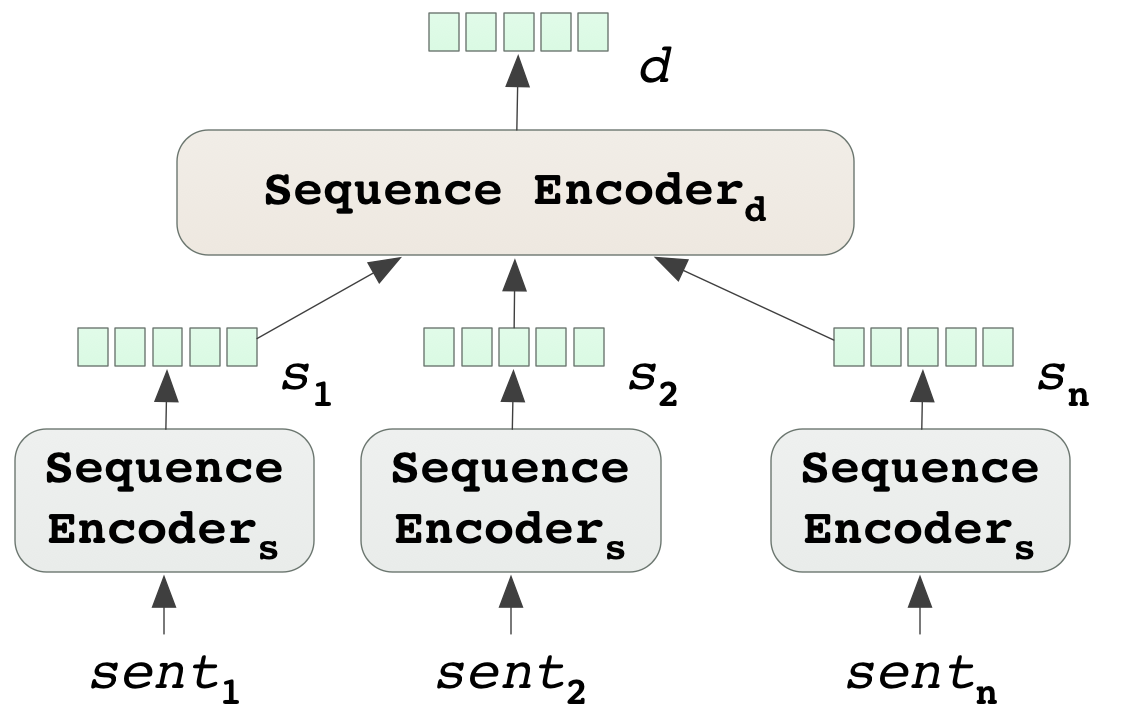
\includegraphics[width=0.4\textwidth]{figures/document_encoder.png}	
\caption{Document Encoder}
\label{fig_doc_encoder}
\end{center}
\end{figure}

\begin{figure}[htbp]
\begin{center}
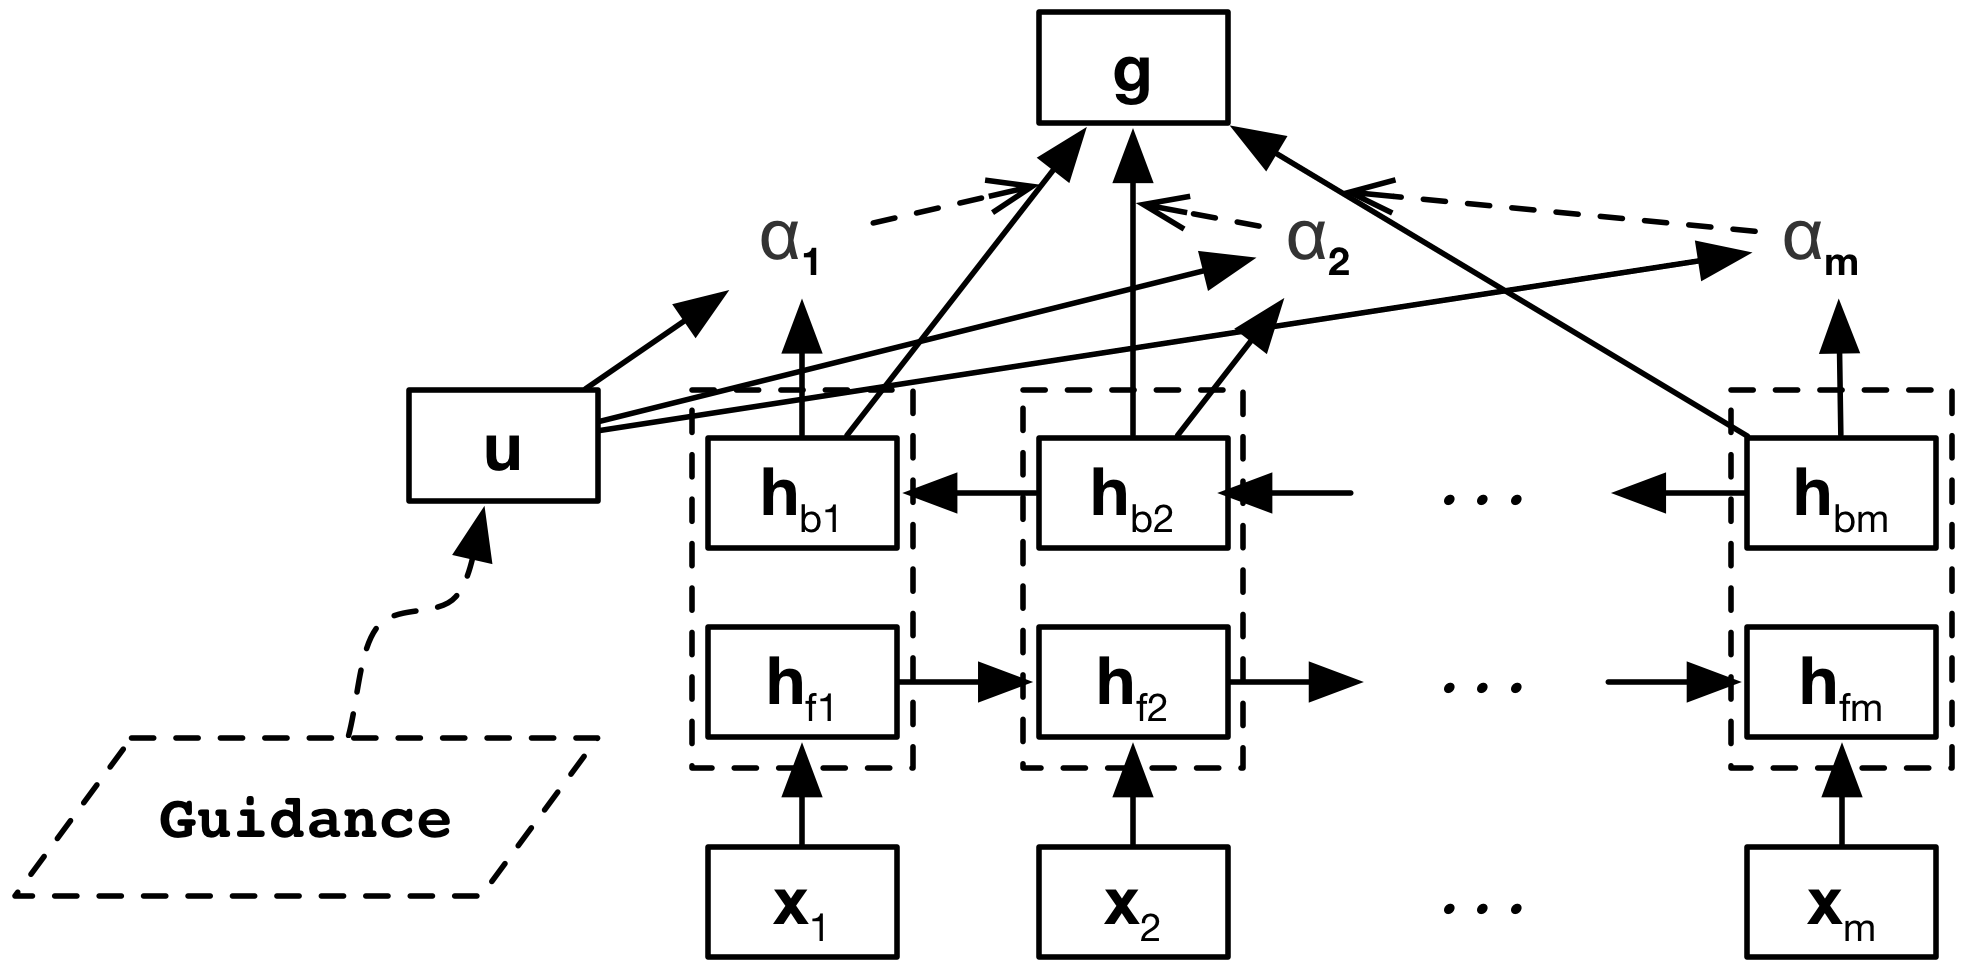
\includegraphics[width=0.45\textwidth]{figures/attentive_seq_encoder.png}	
\caption{Attentive Sequence Encoder}
\label{fig_seq_encoder}
\end{center}
\end{figure}


\paragraph{Bi-GRU Sequence Encoder} 
A prominent challenge in building a sequence encoder is how to take the correlation of each elements into consideration. A promising solution is the bi-directional gated recurrent unit (Bi-GRU) model proposed by \cite{bahdanau2015neural}, which encodes the context of each element by using a gating mechanism to track the state of sequence.
Specifically, Bi-GRU first uses a forward and a backward GRU~\cite{cho2014learning}, which is a kind of Recurrent Neural Network (RNN), to encode the sequence in two opposite directions, and then concatenate the results of both GRUs to form the final outputs. 

Given a sequence $[\mathbf{x}_1, \mathbf{x}_2, ..., \mathbf{x}_T]$ where $\mathbf{x}_t$ is the input embedding of element $t$, the state of Bi-GRU at position $t$ is:

\begin{equation}
%h_t = [\overrightarrow{h}_t , \overleftarrow{h}_t]
\mathbf{h}_t = [\mathbf{h}_{ft}, \mathbf{h}_{bt}]
\end{equation}
where $\mathbf{h}_{ft}$ and $\mathbf{h}_{bt}$ are the states of the forward and backward GRU at position $t$ respectively. The final sequence embedding is either the concatenation of $\mathbf{h}_{fT}$ and $\mathbf{h}_{b1}$, or simply the average of $\mathbf{h}_t$.

% And the state of a single GRU (take forward GRU as an example) is calculated by:
% \begin{equation}
% \mathbf{h}_{ft}=(1-z_t)\odot \mathbf{h}_{f,t-1} + z_t\odot \tilde{\mathbf{h}}_{ft}
% \end{equation}

% \begin{equation}
% \tilde{\mathbf{h}}_{ft}=tanh(\mathbf{W}_h \mathbf{x}_t + r_t\odot \mathbf{U}_h \mathbf{h}_{f,t-1} + \mathbf{b}_h)
% \end{equation}

% \begin{equation}
% r_t=\sigma(\mathbf{W}_r \mathbf{x}_t + \mathbf{U}_r \mathbf{h}_{f,t-1} + b_r)
% \end{equation}

% \begin{equation}
% z_t=\sigma(\mathbf{W}_z \mathbf{x}_t+\mathbf{U}_z \mathbf{h}_{f,t-1} + b_z)
% \end{equation}
% where $\tilde{\mathbf{h}}_{ft}$ is the candidate state of position $t$, $z_t\in{[0,1]}$ is the update gate, $r_t\in{[0,1]}$ is the reset gate, $\mathbf{W}$ and $\mathbf{U}$ are weight matrices, $b$ is the bias, $\odot$ represents element wise product and $\sigma$ corresponds to the sigmoid function. The final sequence embedding is either the concatenation of $\mathbf{h}_{fT}$ and $\mathbf{h}_{b1}$, or simply the average of the average of $\mathbf{h}_t$.

\paragraph{Attentive Sequence Encoder}
\label{sec_att_seq_encoder}
However, $[\mathbf{h}_{fT}, \mathbf{h}_{b1}]$ often fails to capture all the information when the sequence is long, and using the average of $\mathbf{h}_t$ also has the drawback that it treats useless elements equally with informative ones. 

Inspired by \cite{yang2016hierarchical}, we also use a context vector to attentively aggregate the elements, but instead of using a global context vector, we further allow it to be dynamically generated when extra guidance is available (see Section \ref{sec_article_encoder}).


The framework of our attentive sequence encoder is show in Figure \ref{fig_seq_encoder}. Given the Bi-GRU state sequence $[\mathbf{h}_1, \mathbf{h}_2, ..., \mathbf{h}_T]$, we calculate a sequence of attention values $[\alpha_1, \alpha_2, ..., \alpha_T]$ where $\alpha_t \in [0, 1]$ and $\sum_t{\alpha_t}=1$. The final embedding of the sequence $\mathbf{g}$ is then calculated by:
\begin{equation}
\mathbf{g} = \sum_{t=1}^{T}{\alpha_t \mathbf{h}_t}
\label{seq_embed}
\end{equation}
% where the attention value $\alpha_t$ is calculated by:
\begin{equation}
\alpha_t=\frac{exp(\mathbf{v}_t^T \mathbf{u})}{\sum_t{exp(\mathbf{v}_t^T \mathbf{u})}}
\label{gen_att}
\end{equation}
\begin{equation}
\mathbf{v}_t = tanh(\mathbf{W} \mathbf{h}_t)
\label{eq_att_transform}
\end{equation}
where $\mathbf{W}$ is a weight matrix, and $\mathbf{u}$ is the context vector to distinguish informative elements from non-informative ones. 


\subsection{Using Law Articles}
One of the difficulties of using law articles to support our charge prediction lies in the fact that statutory laws contain a large number of law articles, which makes complex classification models time-consuming in training, and run slowly in \orange{production environment} as well. 

We use a two-step approach to resolve this problem. Specifically, at the first step, we use a fast and easy-to-scale classifier to filter out a large fraction of irrelevant articles, and retain the top $k$ articles for the next step. Then, we use neural network to make conprehensive understanding of the top $k$ articles, and then use attention mechanism to select the most relevant ones for charge classification.

\paragraph{Top $k$ Article Extractor}
\label{sec_article_extractor}
We consider the relevant article extraction task as multiple binary classification tasks. Specifically, since 321 distinct law articles in the Criminal Law of the People's Republic of China are mentioned in our dataset, we therefore build 321 binary classifiers where each classifier focuses on the relevance of a specific article. When more articles are considered,
% (e.g. articles in the Anti-Drug Law of the People's Republic of China), 
we can simply add more binary classifiers accordingly, with the existing classifiers untouched.

We use bag-of-words-based SVM as our binary classifier, which is fast and performs well in text classification~\cite{joachims2002learning,wang2012baselines}. Specifically, we use bag-of-words TF-IDF features, chi-square for feature selection and SVM with linear kernel for binary classification. The articles are ranked by the output score and the top $k$ articles are retained for each judgement document.

\paragraph{Article Encoder}
\label{sec_article_encoder}
Since each law article may contain multiple sentences, as shown in Figure \ref{fig_model_framework}, we also use the document encoder described in Section \ref{sec_doc_encoder} to generate the article embedding $\mathbf{a}_j, j\in [1, k]$ for the top $k$ articles. 
While using similar architecure, this document encoder differs from the one used for fact embedding that, instead of using global context vectors, its word-level context vector $\mathbf{u_{aw}}$ and sentence-level context vector $\mathbf{u_{as}}$ are generated dynamically for each case from the fact embedding $\mathbf{d}_f$:
\begin{equation}
\mathbf{u}_{aw} = \mathbf{W}_w \mathbf{d}_f + \mathbf{b}_w;\ \ \ \ \mathbf{u}_{as} = \mathbf{W}_s \mathbf{d}_f + \mathbf{b}_s
\label{eq_dynamic_context_vec}
\end{equation}
where $\mathbf{W}$ is the weight matrix and $\mathbf{b}$ is the bias. 
The context vectors, i.e., $\mathbf{u_{aw}}$ and $\mathbf{u_{as}}$, are then used to produce word-level and sentence-level attention values respectively.
By dynamically generating context vectors, the fact embedding $\mathbf{d}_f$ actually guide the model to attend to informative words or sentences with respect to the facts of each case, rather than just selecting \orange{generally informative ones}.



\paragraph{Attentive Article Aggregator}
The article aggregator aims to generate an aggregated embedding for the top $k$ articles. Since not all the articles are relevant, the difficulty here is how to distinguish relevant articles from irrelevant ones.
% attend more to relevant articles while trying to ignore the irrelevant ones. 

% Due to the inferior classification ability of the relevant article extractor, the order of the top $k$ articles are not \orange{very meaningful}. Therefore, the top $k$ articles are more of a set than a sequence. 
Due to the unreliability of the order of the top $k$ articles, these articles are more of a set than a sequence.
However, as suggested by \cite{vinyals2016matching}, when encoding a set, it is still beneficial to embed the context of each element with a bidirectional RNN.
In our task, specifically, using bi-directional RNN is beneficial to model the co-occurence tendency of relevant articles.

Therefore, we use the attentive sequence encoder in Section \ref{sec_att_seq_encoder} to generate the aggregated article embedding $\mathbf{d}_a$. Again, to guide the attention with fact descriptions, we also dynamicall generate the article-level context vector $\mathbf{u}_{ad}$ by:
% Equation \ref{eq_dynamic_context_vec}, but with another set of parameters.
\begin{equation}
\mathbf{u}_{ad} = \mathbf{W}_d \mathbf{d}_f + \mathbf{b}_d
\end{equation}


\subsection{The Output}
To generate the charge prediction, we first concatenate the document embedding $\mathbf{d}_f$ and the aggregated article embedding $\mathbf{d}_a$, and feed them to two consecutive full connection layers to generate a new vector $\mathbf{d}'$. Then, $\mathbf{d}'$ is passed to a softmax classifier to generate the predicted charge distribution. We use the validation set to determine a threshold $\tau$, and consider all the charges with output probability higher than $\tau$ as positive predictions.
% Note that although other multi-label classification paradigms are also applicable to our problem (see Section \ref{sec_related_work}), we use this method because it performs best in our pilot experiments. 
Also note that the input to the first full connection layer can also be $\mathbf{d}_f$ only, which means we do not use the information from relevant law articles.
% (see comparison in Section \ref{sec_main_results}). 

As for training, we use cross entropy as our loss function:
\begin{equation}
\label{original_loss}
Loss= -\sum_{i=1}^N\sum_{l=1}^L{y_{il} log(o_{il})}
\end{equation} 
where $N$ is the number of training data, $L$ is the number of charges, $y_{il}$ and $o_{il}$ are the target and predicted probability of charge $l$ of datum $i$. Here the target charge distribution $\mathbf{y}$ is generated by setting positive labels to $\frac{1}{m}$ and negative labels to $0$, where $m$ is the number of positive labels.

\paragraph{Supervised Article Attention}
Since the judgement documents also contain gold standard relevant law articles, we can therefore use this information to \orange{supervise} the article attention during training. Specifically, given the top $k$ articles, we want the article attention distribution $\bm{\alpha}\in\mathbb{R}^k$ to simulate the target distribution $\mathbf{t}\in\mathbb{R}^k$, where $t_j=\frac{1}{k'}$ if article $j$ belongs to the gold standard articles and $t_j=0$ otherwise. Here $k'$ is the number of gold standard articles in the top $k$ extractions.

% : \todo{can be simplified}
% \begin{equation}
% t_j=
% \begin{cases}
% 1/|\mathbb{A}|,	& j\in \mathbb{A}\\
% 0,	& else
% \end{cases}
% \end{equation}
% where $\mathbb{A}$ is the set of indices of the gold standard articles in the top $k$ extracted articles, and $|\mathbb{A}|$ is the size of set $\mathbb{A}$. 

We still use cross entropy here, and the loss function is:
\begin{equation}
\label{final_loss}
Loss = -\sum_{i=1}^N(\sum_{l=1}^L{y_{il} log(o_{il})} + \beta \sum_{j=1}^k{t_{ij} log(\alpha_{ij})})
\end{equation}
where $\beta$ is the weight of the article attention loss.


% There are two commonly used methods for multi-label classification in neural network models. The first one is to consider the multi-label classification problem with $L$ labels as $L$ binary classification problem. It uses sigmoid function in the output layer and binary cross entropy as loss function. This method performs well in many multi-label text classification problems \cite{nam2014large}.

% The second method uses the softmax function to generate outputs. It first convert the multi-label target to a probability distribution. For example, suppose there are 4 classes and one datum belongs to class 0 and class 2. This method will convert the $y=[1, 0, 1, 0]$ to $y=[0.5, 0, 0.5, 0]$, and cross entropy will be used as the loss function. After training, a threshold $\tau$ is selected and all the classes that have a score higher than $\tau$ will be considered as positive classes. This method proves to work well in the natural language query classification task \cite{kurata2016improved}. 

% In our pilot experiments, we find that the first method converges about 5 times slower than the second method in our dataset, and the second method also produces better results. We think this phenomenon happens because only a small fraction of our data are multi-label data. Therefore the second method, which uses the same output function as multi-class classification tasks, works better in our task. In this paper, we will use the second method.